\documentclass[11pt,a4paper]{moderncv}
\moderncvstyle{casual}        % Style options: 'casual', 'classic', 'oldstyle', 'banking'
\moderncvcolor{blue}           % Color options: 'blue' (default), 'orange', 'green', 'red', 'purple', 'grey', 'black'

\usepackage[utf8]{inputenc}   % Character encoding
\usepackage[scale=0.9]{geometry}  % Adjust the page margins
\usepackage{graphicx}
\usepackage{hyperref}
\usepackage{tikz}
\usepackage{sourcesanspro} % Use Source Sans Pro for a professional look
\renewcommand{\familydefault}{\sfdefault} % Set sans-serif as default
\usepackage{xcolor} % Add this line for custom colors

% Personal data
\title{} % Suppress default title
\address{Tha Yang District}{Phetchaburi, Thailand}{}
\phone[mobile]{+66~984~580~902}
\email{santosmiguel25@gmail.com}
\homepage{linkedin.com/in/miguelacs}
\social[github]{miguelangelo78}

% Define a dark blue color
\definecolor{mydarkblue}{RGB}{0,56,128}
\definecolor{sectionblue}{RGB}{0,0,128}

%----------------------------------------------------------------------------------
%            Content
%----------------------------------------------------------------------------------
\begin{document}

% Custom header: photo left, name/title, intro, and contacts right
\vspace*{-2em}
\noindent
\begin{minipage}[t]{0.13\textwidth}
  \begin{tikzpicture}
    \clip (0,0) circle (0.5in);
    \node at (0,0) {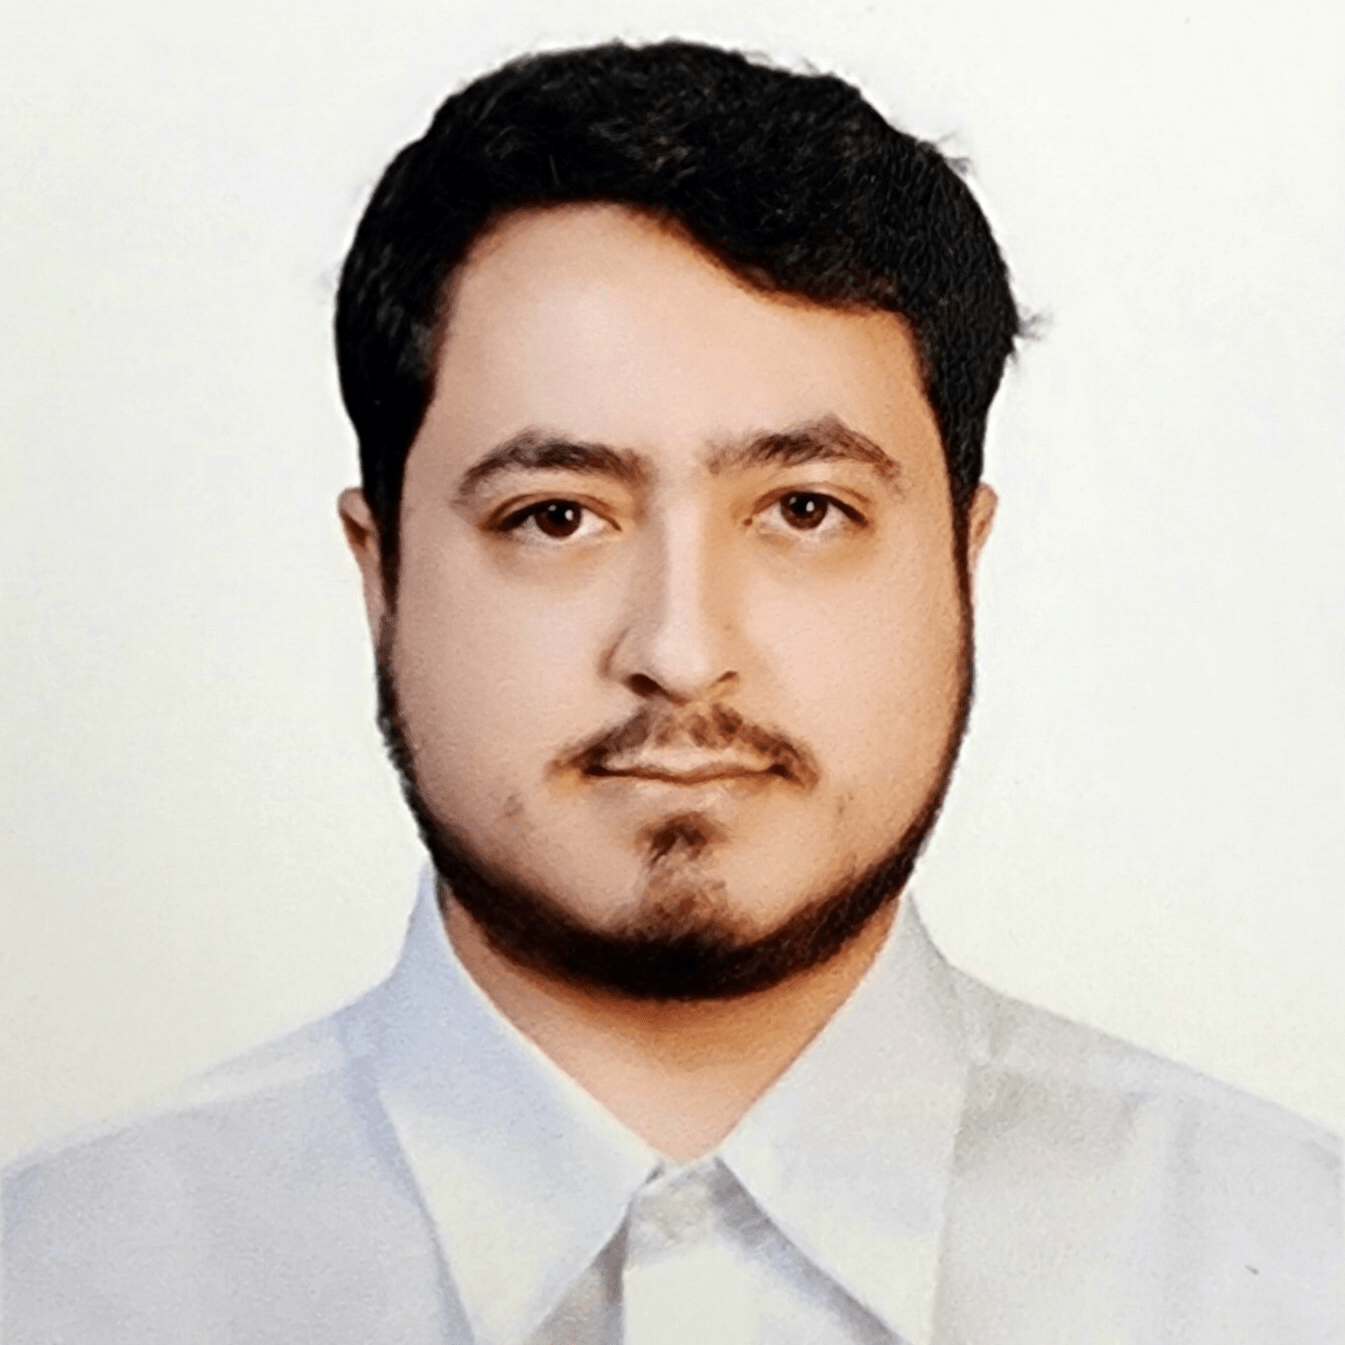
\includegraphics[width=1in]{images/selfie.png}};
  \end{tikzpicture}
\end{minipage}%
\hspace{2em}%
\begin{minipage}[c]{0.80\textwidth}
  \raggedright
  \textbf{\LARGE Miguel Santos | Senior Software Engineer}\\[0.3em]
  Cloud-native software engineer with over 7 years of experience delivering scalable web platforms in AWS using TypeScript, Angular, and Node.js. Proven track record in building microservices, leading greenfield projects, and optimizing developer workflows with Docker and CI/CD. Passionate about clean architecture and user-centered design.\\[0.3em]

  {\footnotesize
    \textit{Seeking a senior software engineering role to build innovative, scalable solutions and contribute to impactful cloud-native projects in a collaborative environment.}
  }\\[0.8em]
  {\footnotesize
    
\includegraphics[height=1em]{images/icon-location.png}
    Phetchaburi City District, Thailand 
    \hspace{0.8em}
    {
\includegraphics[height=1em]{images/icon-whatsapp.png}}
    +66 984 580 902 \\[0.3em]

    {
\includegraphics[height=1em]{images/icon-linkedin.png}}
    \href{https://linkedin.com/in/miguelacs}{linkedin.com/in/miguelacs}
    \hspace{0.8em}
    {
\includegraphics[height=1em]{images/icon-email.png}}
    \href{mailto:santosmiguel25@gmail.com}{santosmiguel25@gmail.com}
    \hspace{0.8em}
    {
\includegraphics[height=1em]{images/icon-github.png}}
    \href{https://github.com/miguelangelo78}{github.com/miguelangelo78}
  }
\end{minipage}

\section{Work Experience}
\vspace{-1em}

% Hubexo
\begin{minipage}[c]{0.08\textwidth}
  \raggedleft
  \raisebox{-3em}{
\includegraphics[height=2em]{images/icon-hubexo.jpeg}}
\end{minipage}%
\hspace{0.5em}%
\begin{minipage}[t]{0.95\textwidth}
  \textbf{Senior Software Developer} \,•\, {\color{mydarkblue}Hubexo}\\
  {\footnotesize Jan 2022 -- Present}
  \begin{itemize}
    \item Develop responsive cloud-native Web Apps using TypeScript, Angular, Node.js, and Docker on AWS.
    \item Integrate AI systems into applications to enhance user experience and functionality.
    \item Design CI/CD workflows to streamline QA deployments.
    \item Architected and shipped a modular OpenSearch engine with custom indexing and ranking logic.
  \end{itemize}
\end{minipage}
\vspace{0.5em}

% Apak Group Limited
\begin{minipage}[c]{0.08\textwidth}
  \raggedleft
  \raisebox{-3em}{
\includegraphics[height=2em]{images/icon-apak.png}}
\end{minipage}%
\hspace{0.5em}%
\begin{minipage}[t]{0.9\textwidth}
  \textbf{Software Developer} \,•\, {\color{mydarkblue}Apak Group Limited}\\
  {\footnotesize Apr 2020 -- Nov 2021}
  \begin{itemize}
    \item Implemented scalable backend microservices in AWS using TypeScript and Node.js.
    \item Built frontend applications using .NET/C\# integrated with Azure DevOps pipelines.
    \item Led the delivery of major features for financial proposal settlements.
  \end{itemize}
\end{minipage}
\vspace{0.5em}

% Gamma
\begin{minipage}[c]{0.08\textwidth}
  \raggedleft
  \raisebox{-3em}{
\includegraphics[height=2em]{images/icon-gamma.png}}
\end{minipage}%
\hspace{0.5em}%
\begin{minipage}[t]{0.9\textwidth}
  \textbf{Graduate Software Analyst/Developer} \,•\, {\color{mydarkblue}Gamma}\\
  {\footnotesize Jul 2018 -- Apr 2020}
  \begin{itemize}
    \item Designed and built backend/frontend components using Java, SQL Server, and Apache Struts.
    \item Improved interoperability via Single Sign-On integration.
    \item Developed backend services for telecom switching using STAC and PAC codes.
  \end{itemize}
\end{minipage}
\vspace{0.5em}

% Replace Education and Languages with a single row of minipages, each half the page width
\begin{minipage}[t]{0.6\textwidth}
  \section{Education}
  % Entry 1
  \begin{minipage}[t]{0.13\textwidth}
    \raggedleft
    \raisebox{-1.5em}{
\includegraphics[height=2.5em]{images/icon-usw.png}}
  \end{minipage}%
  \hspace{0.3em}%
  \begin{minipage}[t]{0.9\textwidth}
    2014 -- 2018\\
    \textbf{MEng Computer Systems Engineering}\\
    University of South Wales, UK\\[-0.5em]
    \begin{itemize}
      \item Graduated with distinction.
      \item Master's thesis: designed and developed a CPU architecture for a soft microprocessor.
    \end{itemize}
  \end{minipage}
\end{minipage}%
\hfill
\begin{minipage}[t]{0.4\textwidth}
  \section{Languages}
  \cvitem{\textbf{Portuguese}}{Native}
  \cvitem{\textbf{English}}{Bilingual}
  \cvitem{\textbf{Spanish}}{Intermediate}
  \cvitem{\textbf{Thai}}{Beginner}
\end{minipage}

\section{Technical Skills}
\cvitem{\textbf{Languages:}}{TypeScript, JavaScript, Python, Java, C\#, Bash}
\cvitem{\textbf{Frameworks:}}{Node.js, Angular, Next.js, NestJS, .NET}
\cvitem{\scriptsize\textbf{DevOps \& Cloud:}}{AWS, Docker, CI/CD, Azure DevOps}
\cvitem{\textbf{Databases:}}{PostgreSQL, SQL Server}
\cvitem{\textbf{Search \& AI:}}{OpenSearch, AI integration (LLMs, embeddings)}

\section{Projects}
{
\cvitem{\textbf{Coinflake:}}{Financial investment tracking app for crypto, stocks, and commodities. Built with Next.js and PostgreSQL, featuring dynamic data visualizations via Lightweight Charts.}
\cvitem{\textbf{Swapper:}}{Web app enabling Thai teachers to find swap opportunities for job relocation. Built with Next.js and Tailwind; authentication via NextAuth; deployed on Vercel. 50+ teachers registered. {\color{mydarkblue}\href{https://swapper-beta.vercel.app}{Website}}}
\cvitem{\textbf{Structura:}}{Experimental meta programming language for structured AI prompts. {\color{mydarkblue}\href{https://github.com/miguelangelo78/structura}{GitHub}}}
}

\end{document}
